
%!TEX ROOT=ctutest.tex

\chapter{Existující řešení}
\label{chap:existujici-reseni}

V následující kapitole rozeberu konkurenční systémy, které se již pokouší požadovanou funkcionalitu implementovat. U každého z nich zmíním nejprve obecné informace k čemu slouží a následně se zaměřím na jejich klady a zápory. Zároveň bych rád zmínil, že u některých systémů nebylo zrovna snadné si je vyzkoušet a provést nějakou analýzu. Důvodem je to, že ne všechny zmiňované systémy jsou zdarma a přístupné široké veřejnosti. Abych uvedl příklad, tak Google Classroom je možné využívat pouze skrz školní účet registrovaný u některé školy, která si tento systém platí. Podobný problém je i pro většinu dalších systémů. Tuto nepříjemnost jsem řešil většinou tak, že jsem vycházel například z různých návodů pro užívání těchto systémů dostupných na internetu.






\section{Microsoft Teams}

V současné době pro nás, jakožto studenty ČVUT, velmi známý a hojně využívaný nástroj. Ukázku uživatelského rozhraní lze vidět na obrázku \ref{img:teams}.

Rozhodně tedy patří k těm populárnějším, a to nejen ve školách, ale zejména i ve firemní sféře. Jedná se totiž o produkt z dílny Microsoftu, díky čemuž nabízí nadstandardní možnosti integrace s dalšími nástroji jako například cloudové úložiště, poznámkové bloky a hlavně umožňuje napřímo editovat dokumenty ve formátu .docx.

Samozřejmě jej lze doplnit i o další pluginy jako například Microsoft Planner pro plánování nejrůznějších úkolů a podobně.

Všechno toto lze samozřejmě považovat za obrovskou výhodu, a to převážně v již zmiňovaných firmách. Nebo obecně tam, kde si lidé s takto komplexním nástrojem poradí. Například tedy i vysoké či některé střední školy.

Tak velké množství funkcí se ovšem může stát nevýhodou v těch oblastech, kde je vyžadována spíše jednoduchost a co nejvyšší uživatelská přívětivost, a to rozhodně základní školy jsou. Takoví uživatelé ocení spíše systém, přesně šitý na míru jejich potřebám. Budou rádi, když nebudou muset nikde nastavovat žádné oprávnění a podobné věci. Nakonec by také mohli mít problém s vícero Microsoft účty, mezi kterými by potřebovali přepínat. Například pracovní a osobní.

\begin{figure}[H]
    \caption{Ukázka uživatelského rozhraní Microsoft Teams, vlastní screenshot}
    \centering
    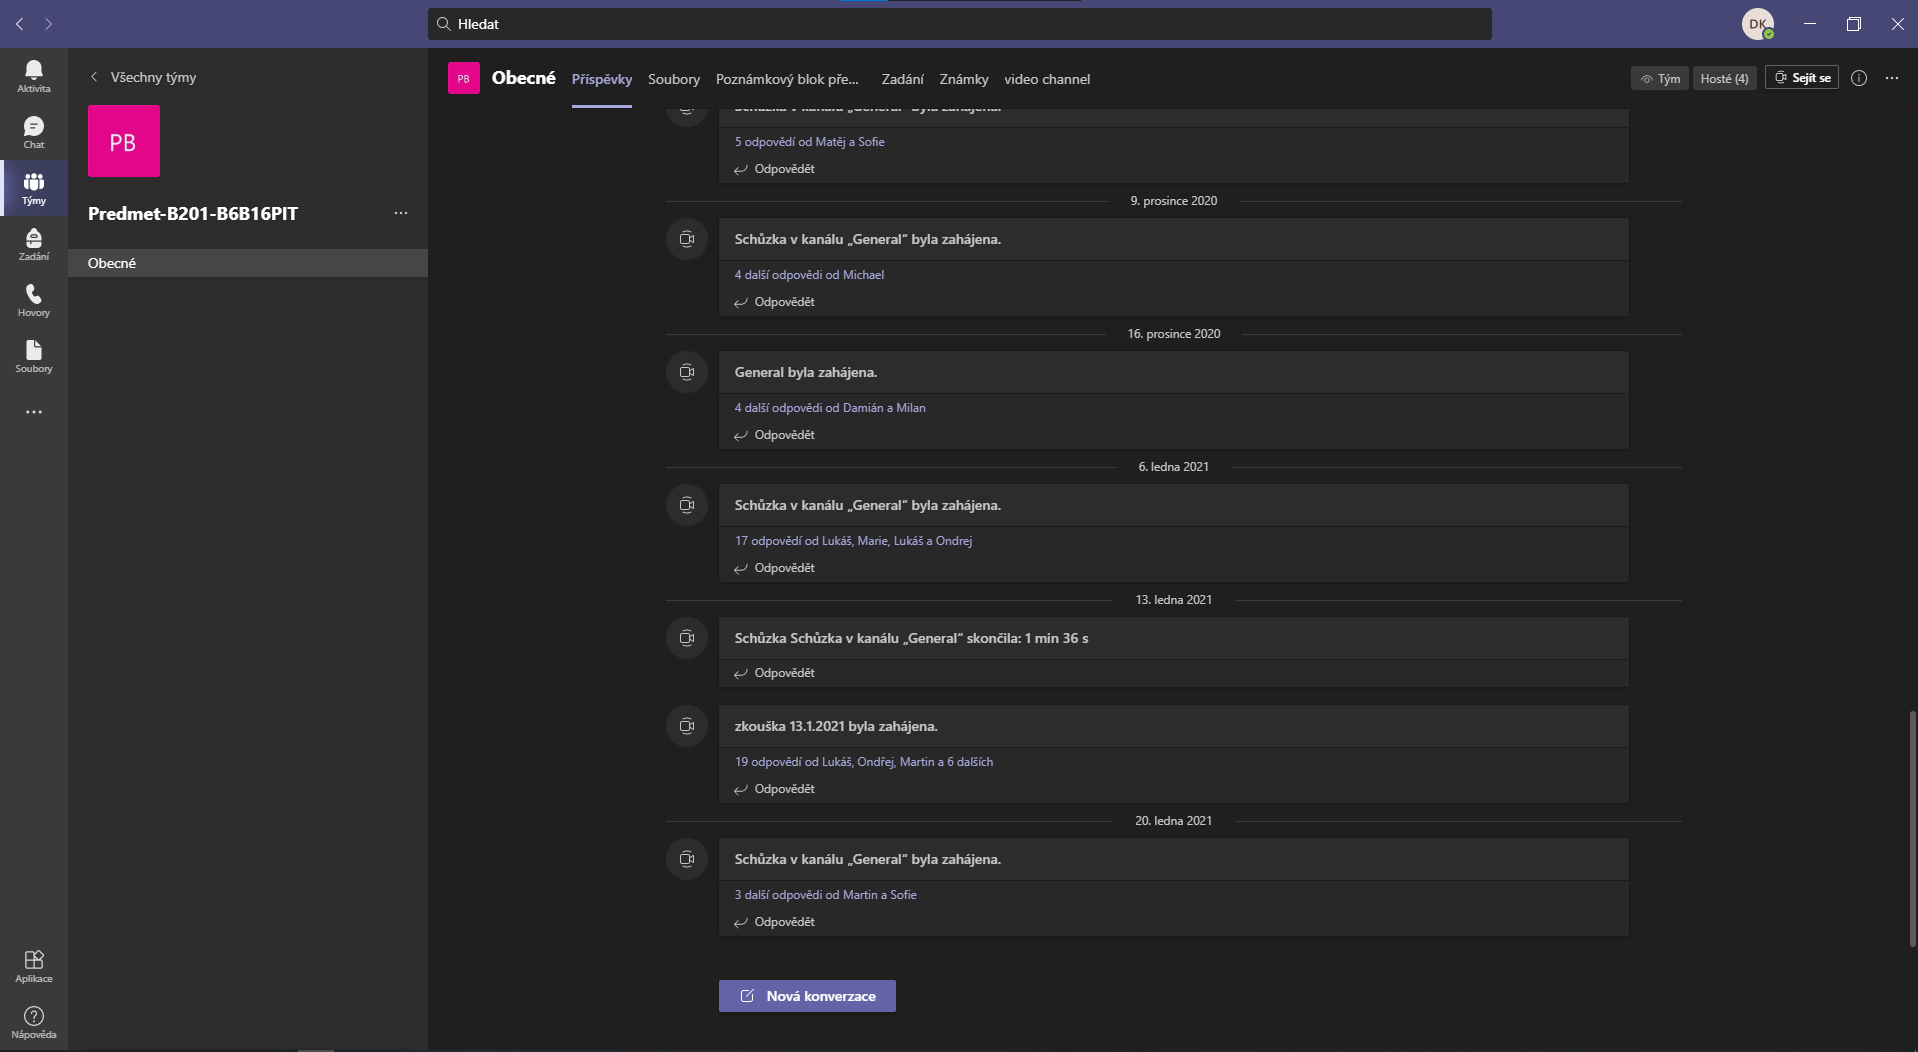
\includegraphics[width=\textwidth]{images/teams}
    \label{img:teams}
\end{figure}

Za výhody lze tedy považovat:
\begin{itemize}
  \item Vysoká možnost integrace s dalšími nástroji
  \begin{itemize}
    \item MS Office
    \item OneNote
    \item OneDrive
    \item a další...
  \end{itemize}
  \item Podpora velké firmy a kvalitní zázemí
  \item Poměrně rozšířený a prozkoušený systém.
  \item Dostupná mobilní aplikace
\end{itemize}

Na druhou stranu, nedostatky jsou například:
\begin{itemize}
  \item Přílišná komplexnost vzhledem k základním školám (nabízí příliš mnoho nepotřebných možností a funkcí)
  \item Naopak postrádá například propracovanější systém pro odevzdávání a kontrolu úkolů
  \item Nedostatečné možnosti nastavení práv
    \begin{itemize}
    \item Skrýt některé kanály v týmu pro určité uživatele
    \item Vymezit pro hosta, co přesně může a nemůže vidět
  \end{itemize}
  \item Nutnost vytvářet si sám strukturu týmů a skupin. Toto často vede k nekonzistentním stavům, kde například každý předmět je trochu jinak uspořádaný a uživatel je poté velmi zmatený.
  \item Při posílání dokumentů je zde potřeba myslet na adresářovou strukturu, aby zůstal obsah přehledný. Toho nemusí být malé děti schopné a i pro dospělé to může být obtěžující.
\end{itemize}


\section{Google Classroom}

O něco více se potřebám škol snaží přiblížit platforma Google Classroom. Ukázku jejího rozhraní lze vidět na obrázku \ref{img:google_classroom}. Nicméně i ta má několik nedostatků.

Abych začal výhodami, tak musím zmínit poměrně čisté a hezké uživatelské rozhraní, které i přes svou jednoduchost nabízí spoustu skvělých funkcí.

Učitel má možnost vytvářet nové kurzy, do kterých může přidávat témata s jednotlivými úkoly nebo může jen psát příspěvky.

Do těchto kurzů se musí žáci přihlašovat sami pomocí kódu. Už to by se dalo považovat za nevýhodu, protože sice se může zdát, že to ušetří práci učiteli, nicméně dovedu si představit, že s tím některý žák bude mít problém a ve finále učitel stejně žádný čas neušetří, protože bude muset žákovi pomoct se do kurzu dostat. V tomto ohledu se mi tedy jeví jako lepší varianta to, že žák dostane již vytvořený účet, který je připojen do všech předmětů ve třídě.

Výhodou může být integrace s dalšími nástroji od společnosti Google. Například Google dokumenty, tabulky, Google disk a podobně. Nicméně i to s sebou nese spoustu problémů, které popisuji v dalším odstavci.

Mezi velké nevýhody patří to, že se uživatel musí přihlašovat svým školním Google účtem. Z toho plyne několik problémů. Jednak jsem se často setkal s uživateli, kteří ani nevědí, že nějaký Google účet mají. Ale mnohem horší je pak přepínání účtů. Téměř každý uživatel má, ať už nevědomky nebo vědomě, svůj osobní Google účet, ale najednou se musí přihlašovat pomocí jiného. Už to může být pro velkou část uživatelů dost zmatečné, a navíc se k tomu pak přidají podobné problémy například při použití Google disku nebo Google dokumentů či fotek. Uživatel je například na svém mobilním telefonu přihlášen pod svým osobním účtem, něco vyfotí, myslí si, že to najde na počítači ve svých Google fotkách, ale pod jiným účtem tyto fotky nenajde.

\begin{figure}[H]
    \caption{Ukázka uživatelského rozhraní Google Classroom, převzato z \cite{google_classroom}}
    \centering
    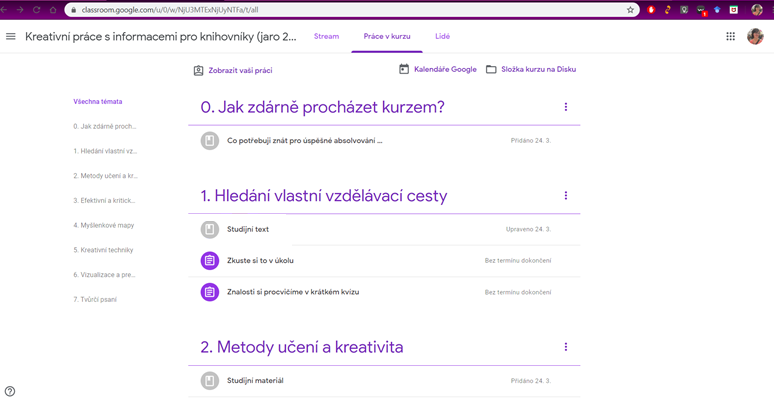
\includegraphics[width=\textwidth]{images/google_classroom}
    \label{img:google_classroom}
\end{figure}

Výhody jsou tedy podobné jako u MS Teams:
\begin{itemize}
  \item Integrace s dalšími Google nástroji
  \begin{itemize}
    \item Google fotky
    \item Google dokumenty, tabulky
    \item Google disk
    \item a další...
  \end{itemize}
  \item Podpora velké společnosti a kvalitní zázemí
  \item Poměrně rozšířený a zaběhlý systém
  \item Čisté a moderní uživatelské rozhraní
  \item Dostupná mobilní aplikace
\end{itemize}

Ovšem i zde existují nedostatky:
\begin{itemize}
  \item Přepínání Google účtů (osobní, školní)
  \item Žáci se musí dostat do kurzů sami
  \item Odevzdávání řešení
  \begin{itemize}
    \item Žák může buď psát přímo do zadání, pak si ho ale může, byť jen omylem, změnit.
    \item Nebo může mít práva zadání pouze zobrazit. Pak je pro něj ale situace složitější v tom, že musí vytvořit nový dokument a poradit si s formou sám. Buď zadání zkopíruje a dopisuje do něj nebo se na otázky nějak odkazuje např. čísly.
  \end{itemize}
  \item Nepropracované multiple choice úkoly v porovnání např. s Moodle (chybí kupříkladu poměrné bodové hodnocení za částečné řešení)
\end{itemize}

\section{Bakaláři}

Nyní už se dostávám k nástroji, který se skutečně snaží pokrýt potřeby škol. Uživatelům poskytuje nepřeberné množství funkcí včetně například plánovaných akcí školy, knihovny, suplování a další. Právě tyto, z mého pohledu, trochu nadbytečné funkce činí ovšem tento systém hovorově řečeno "přeplácaný" jak lze vidět na ukázce \ref{img:bakalari}.

Samozřejmě netvrdím, že je to úplně špatně. Tento nástroj je přeci jen stavěn spíše pro kompletní pokrytí všech požadavků škol, což splňuje dobře. Nicméně předmětem mé práce je přijít s řešením, které bude velmi jednoduché a intuitivní pro všechny druhy uživatelů a to jde trochu proti sobě s pokrytím všech myslitelných požadavků.

S předchozím bodem také souvisí historický vývoj této platformy, která byla původně koncipována jako desktopová aplikace. V současné době je ovšem zájem spíše o webové rozhraní, a tak vzniká nekonzistence mezi těmito dvěma prostředími. Jednak vypadají rozdílně, a navíc poskytují rozdílné funkcionality, což může být velice matoucí.

Také je nutno podotknout, že systém Bakaláři je v některých ohledech vcelku "nedotažený". Například bych rád zmínil proces zadávání a schvalování úkolů. Ze sesbíraných referencí vím, že učitelé často zapomenou označit úkol za dokončený, když ho odevzdají všichni studenti. Pak se stává to, že ho i nadále všichni studenti vidí ve svém seznamu úkolů a časem se z tohoto seznamu stane nepořádek. Lepší by bylo, kdyby se žákovi úkol po schválení přestal zobrazovat v seznamu a případně se přesunul do nějakého méně nápadného seznamu odeslaných či hotových úkolů. Učitel by pak viděl úkol také jen do té doby než ho dořeší všichni studenti a následně by se automaticky označil jako dokončený a také by se přesunul do jiného seznamu.

\begin{figure}[H]
    \caption{Ukázka uživatelského rozhraní Bakaláři, převzato z \cite{bakalari}}
    \centering
    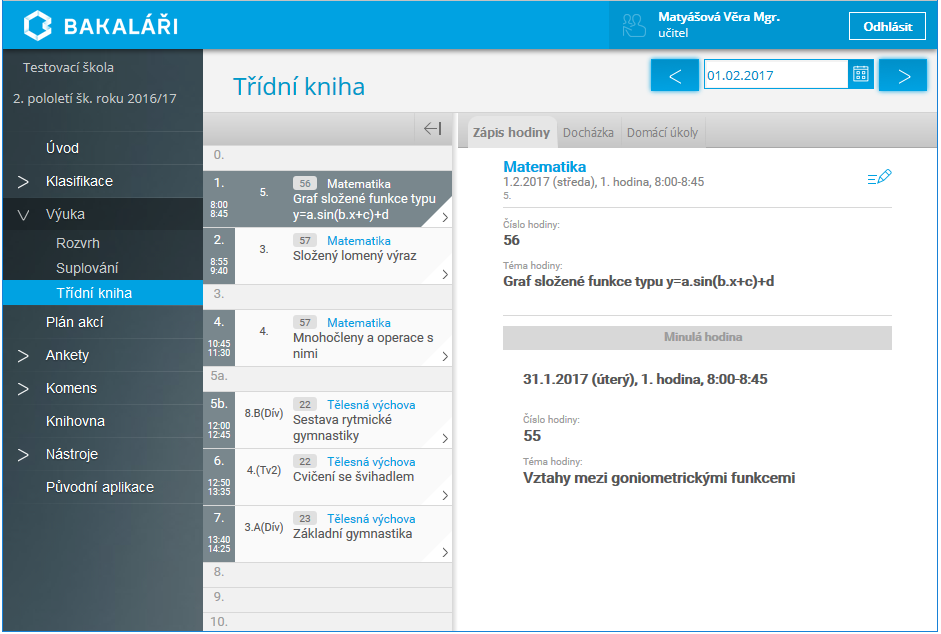
\includegraphics[width=\textwidth]{images/bakalari}
    \label{img:bakalari}
\end{figure}

Výhody:
\begin{itemize}
  \item Snaha o kompletní pokrytí všech požadavků škol
  \item Dostupné výukové materiály pro práci se systémem
  \item Dostupná mobilní aplikace
  \item Vhodné spíše pro úplnou digitalizaci školy
\end{itemize}

Nedostatky:
\begin{itemize}
  \item Náročnější k naučení se všech možných funkcí
  \item Příliš komplexní (vzhledem k požadavku na co největší jednoduchost nabízí tento systém příliš nepotřebných funkcí, například akce školy, knihovny, atd.)
  \item V některých částech "nedotažené" (např. splnění úkolu)
  \item Různý vzhled a funkce na různých platformách (zejména desktopová a webová aplikace)
  \item Často padá či nefunguje.
  \begin{itemize}
      \item To může být způsobeno historicky použitím různých programovacích jazyků a technologií
  \end{itemize}
\end{itemize}


\section{Škola OnLine}

Tato platforma je poměrně dost podobná zmiňovaným Bakalářům. Možná i to je důvod proč se tyto platformy v roce 2019 spojily. Také se snaží pokrýt většinu požadavků škol a i když není zatím tolik komplexní, také je poměrně těžkopádná. Ukázku uživatelského rozhraní lze vidět na obrázku \ref{img:skolaonline}

\begin{figure}[H]
    \caption{Ukázka uživatelského rozhraní Škola OnLine, převzato z \cite{skolaonline}}
    \centering
    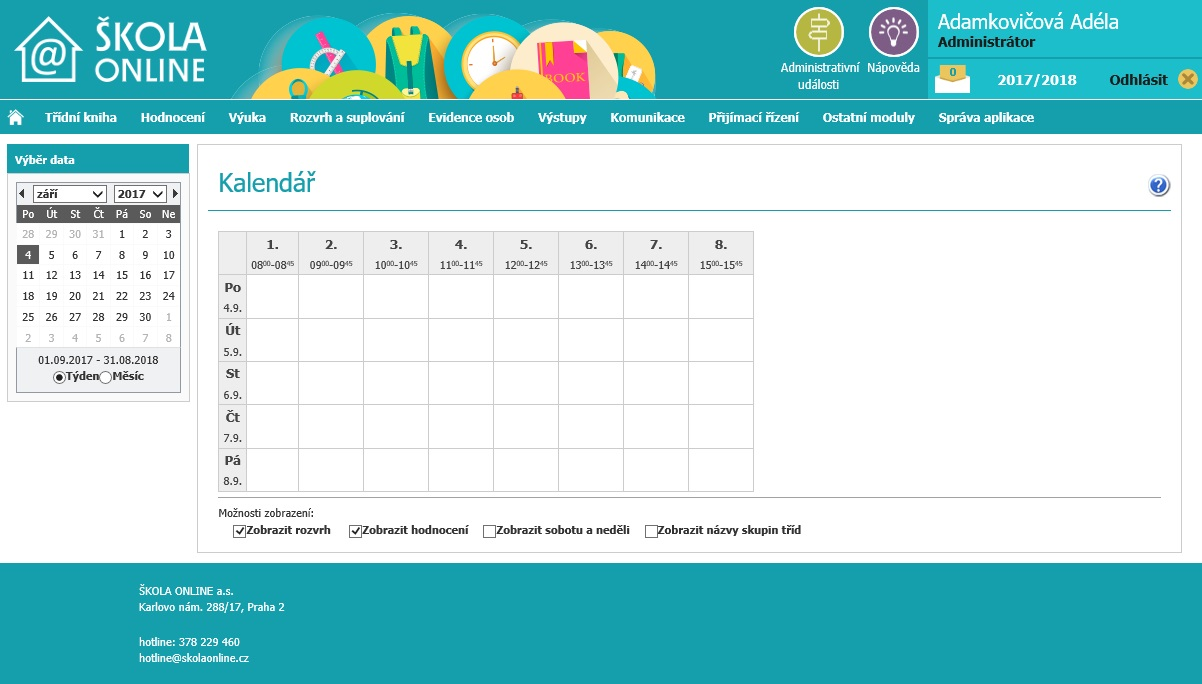
\includegraphics[width=\textwidth]{images/skola_online}
    \label{img:skolaonline}
\end{figure}
\newpage
Výhody:
\begin{itemize}
  \item Snaha o kompletní pokrytí všech požadavků škol
  \item Dostupné výukové materiály pro práci se systémem
  \item Dostupná mobilní aplikace
  \item Vhodné spíše pro úplnou digitalizaci školy
\end{itemize}

Nedostatky:
\begin{itemize}
  \item Příliš komplexní (podobně jako Bakaláři, tak i Škola OnLine nabízí vzhledem k požadavku na co nejvyšší jednoduchost příliš nepotřebných funkcí, například knihovna, školní akce)
  \item Neintuitivní uživatelské rozhraní (Pomohly by například jen drobnosti jako, aby názvy úkolů a podobné nápisy fungovaly jako odkazy)
\end{itemize}


\section{Škola v pyžamu}

Poměrně hezkým projektem je Škola v pyžamu, jehož uživatelské rozhraní lze vidět na obrázku \ref{img:skola_v_pyzamu}. Zde se autoři snaží právě o jednoduchost, kterou rodiče a malé děti ocení nejvíce. Nicméně zde na druhou stranu zase několik věcí chybí. Například učitel si nemůže psát k žákům různé poznámky či nevidí přehledné shrnutí všech úkolů. Vidí pouze úkoly pod sebou a u každého z nich seznam žáků se stavem vypracování. Také by bylo vhodnější rozdělení na jednotlivé předměty a snazší přepínání tříd pro učitele.

\begin{figure}[H]
    \caption{Ukázka uživatelského rozhraní Škola v pyžamu, převzato z \cite{skola_v_pyzamu}}
    \centering
    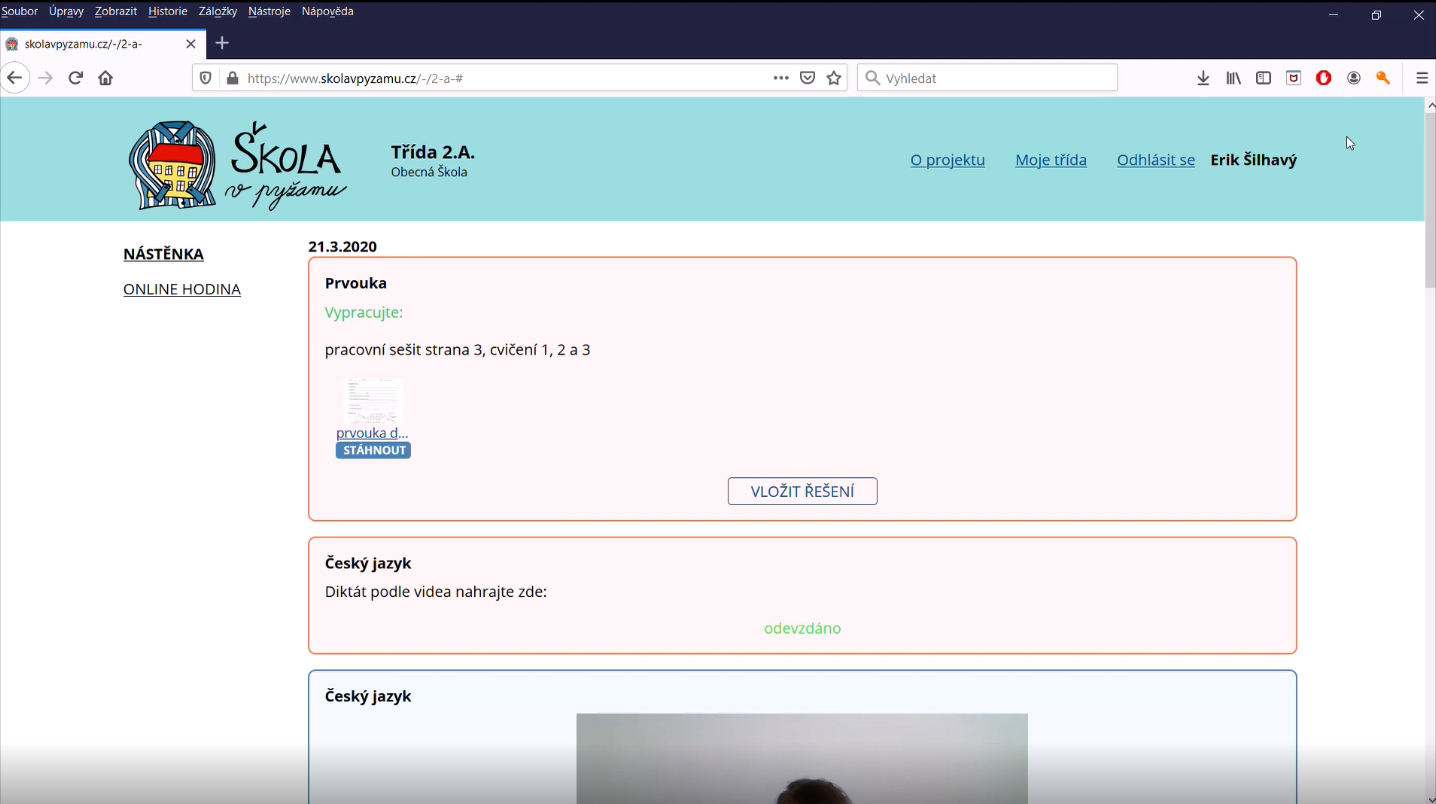
\includegraphics[width=\textwidth]{images/skola_v_pyzamu}
    \label{img:skola_v_pyzamu}
\end{figure}

Výhody:
\begin{itemize}
  \item Velmi jednoduché prostředí (dáno ovšem absencí některých funkcí)
  \item Zdarma
\end{itemize}

Nedostatky:
\begin{itemize}
  \item Chybí mobilní aplikace
  \item Chybí lepší rozdělení jednotlivých předmětů
  \item Složité přepínání mezi třídami
\end{itemize}


\section{Moodle}

Tento systém je znám spíše na vysokých školách. Jedná se o poměrně komplexní nástroj, který umožňuje i tvorbu testů různých druhů, systém známkování, multijazyčnost a další. Nicméně, jak již vyplývá z faktu, kde se využívá, není jeho využití pro základní školy příliš vhodné. Přeci jen není tolik intuitivní, jak by bylo potřeba. Navíc je vhodné pro jeho konfiguraci mít k dispozici IT odborníka, kterých nebývá na základních školách dostatek. Ukázku jeho uživatelského rozhraní lze vidět na obrázku \ref{img:moodle}.

\begin{figure}[H]
    \caption{Ukázka uživatelského rozhraní Moodle, vlastní screenshot}
    \centering
    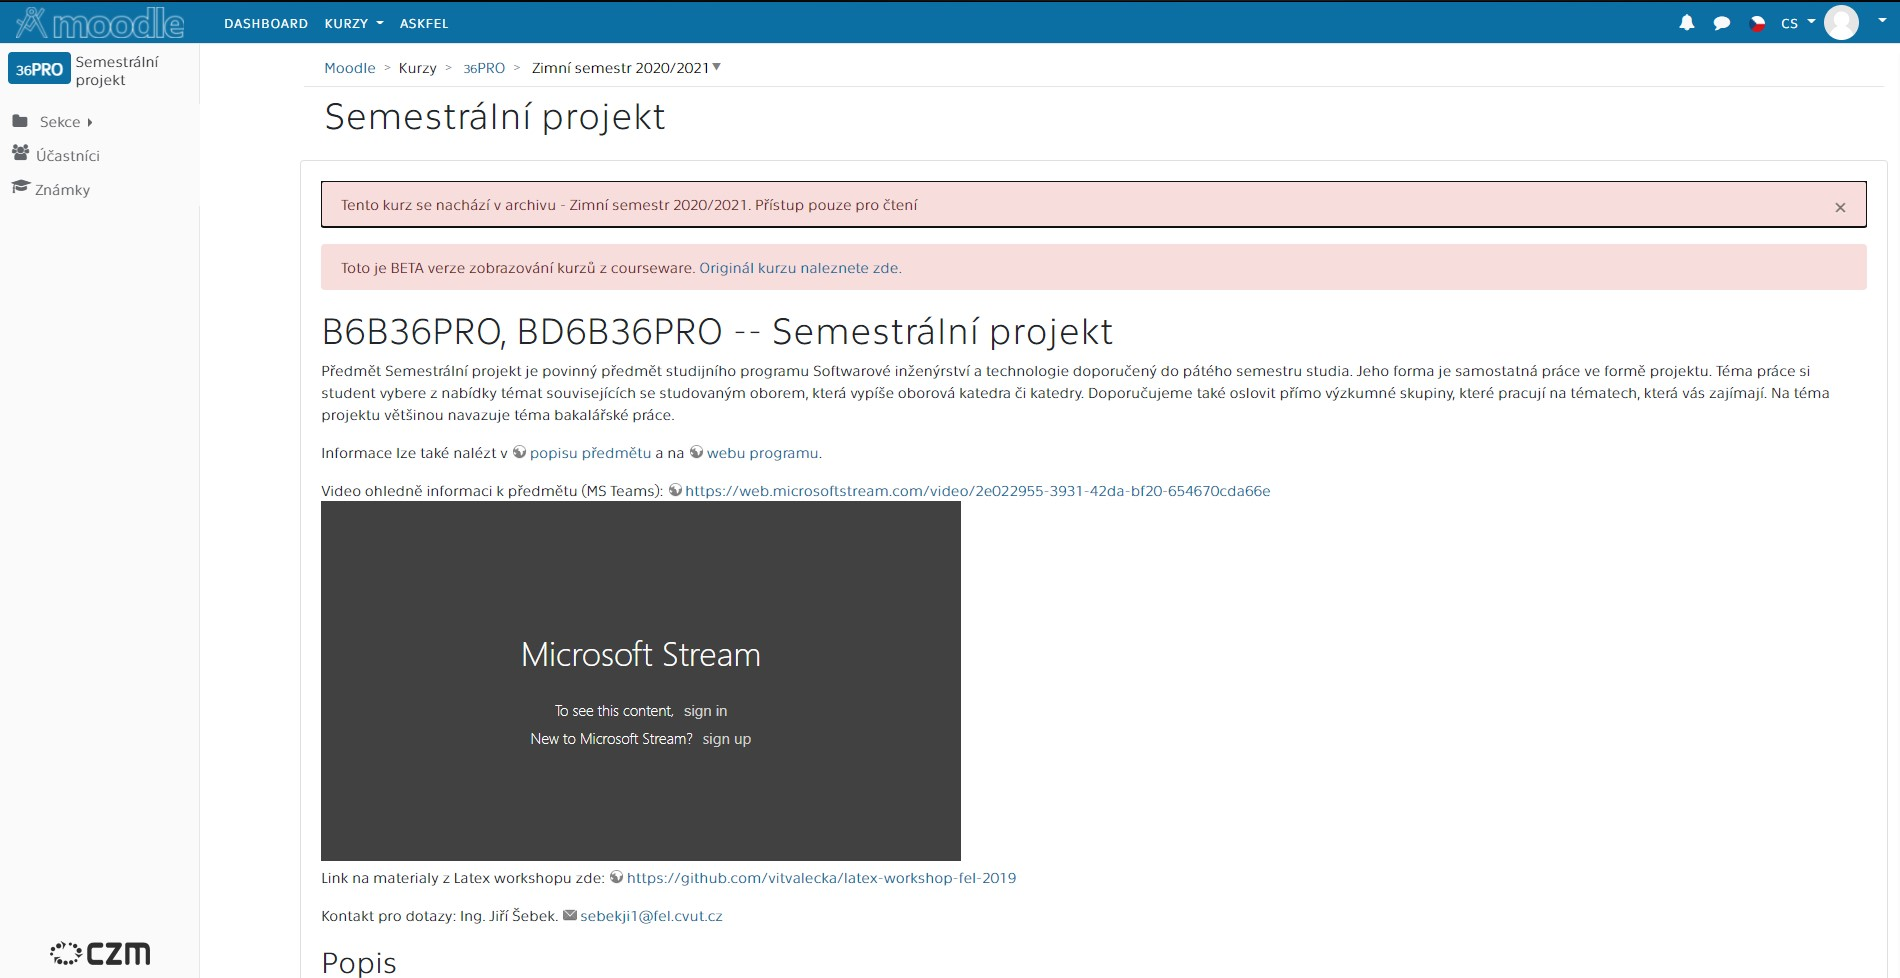
\includegraphics[width=\textwidth]{images/moodle}
    \label{img:moodle}
\end{figure}

Výhody:
\begin{itemize}
  \item Poměrně dobré možnosti tvorby online testů
  \begin{itemize}
    \item Průběžné odesílání řešení pomocí AJAX
    \item Možnost nastavit poměrné bodové hodnocení částečně správných řešení
  \end{itemize}
  \item Různé role uživatelů
\end{itemize}

Nedostatky:
\begin{itemize}
  \item Nepříliš intuitivní
  \begin{itemize}
      \item Například na úvodní stránce by bylo dobré u každého předmětu vidět přehled toho, co je potřeba udělat.
  \end{itemize}
  \item Má problémy na mobilních zařízeních, kde někdy dokonce není vidět část obsahu.
  \item Složitější konfigurace
\end{itemize}

\section{Online cvičení}

Tento web je zaměřen trochu jinak. Je vhodný spíše pro procvičování různých typů cvičení. Žák zde nalezne spoustu dostupných úkolů, ale tím výhody v podstatě končí. Celkově systém není příliš "dotažený". Například přidávání do skupin probíhá zbytečně složitým způsobem, kdy se žák musí sám registrovat, vyhledat podle kódu skupinu, žádat admina o přidání a pak doufat, že ho admin přidá. Mnohem jednodušší se mi jeví řešení, kdy toto vše vyřídí za žáky sám učitel. Ukázku tohoto webu lze vidět na obrázku \ref{img:onlinecviceni}.


\begin{figure}[H]
    \caption{Ukázka uživatelského rozhraní Online cvičení \cite{onlinecviceni}, vlastní screenshot}
    \centering
    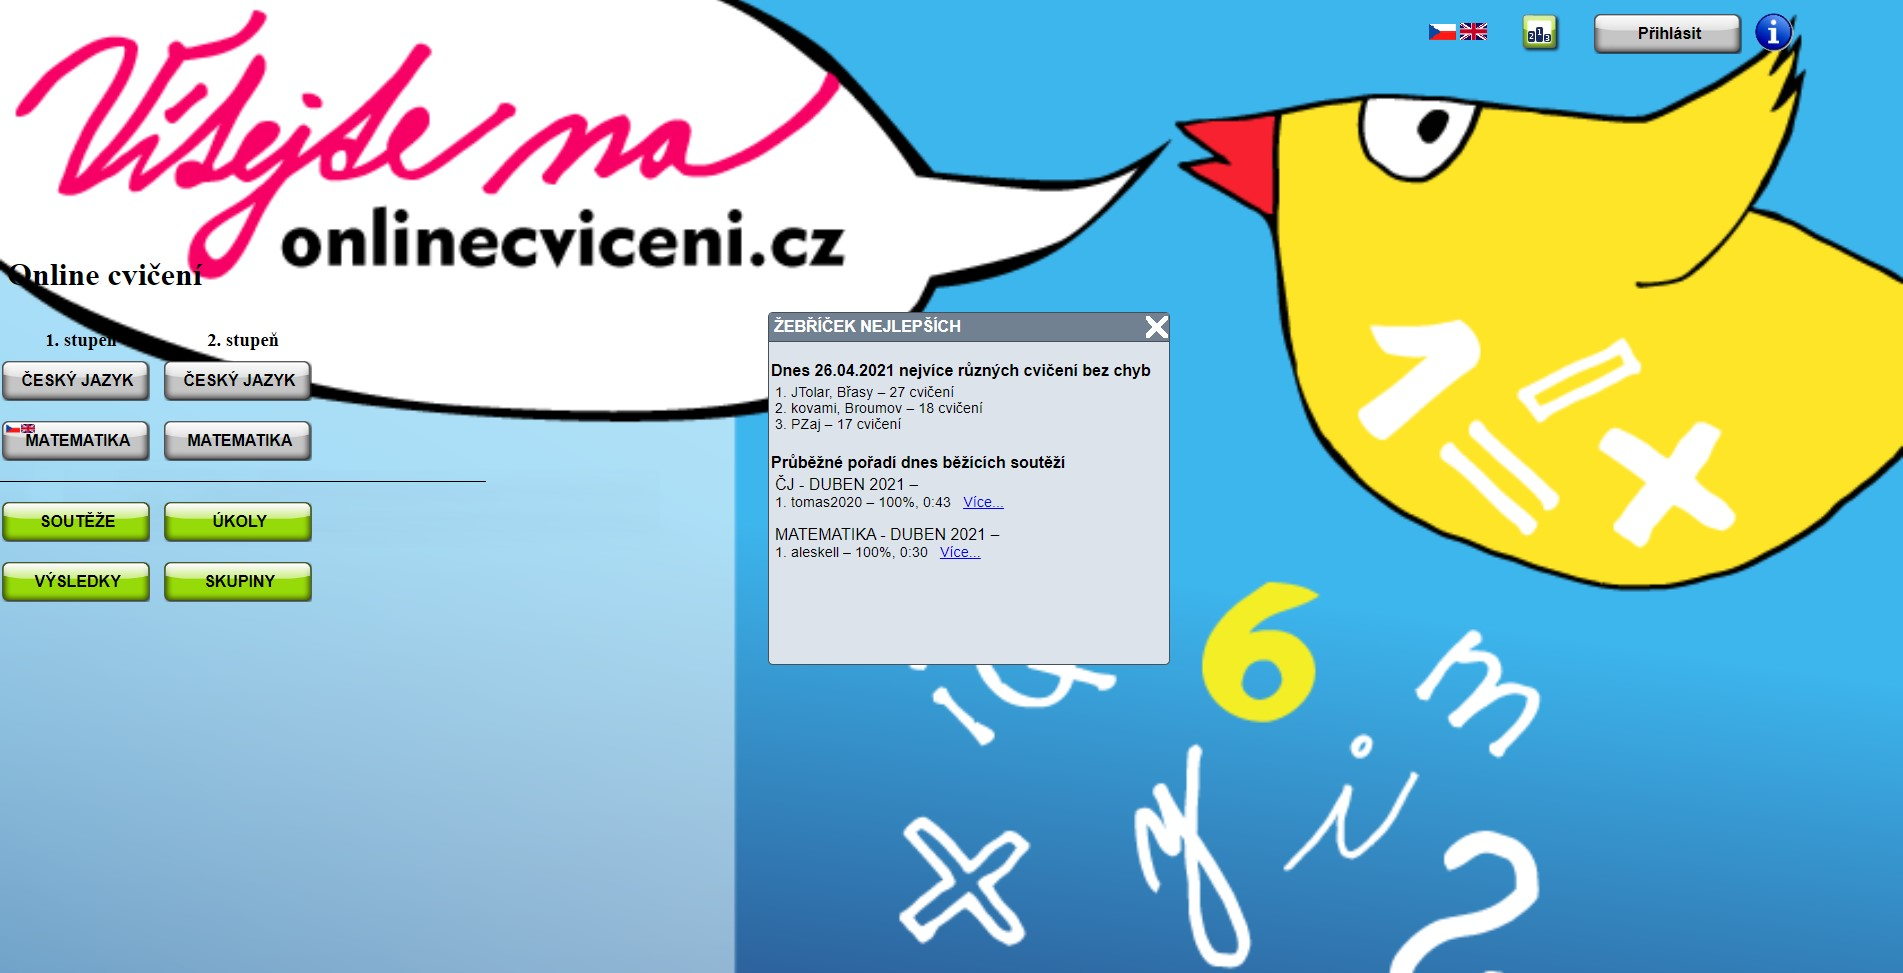
\includegraphics[width=\textwidth]{images/onlinecviceni}
    \label{img:onlinecviceni}
\end{figure}

Výhody:
\begin{itemize}
    \item Velké množství obsahu (různá cvičení)
\end{itemize}

Nedostatky:
\begin{itemize}
    \item Nedotažené (zbytečně složité a nepřehledné vzhledem k tak malému počtu funkcí)
    \item V dnešní době odrazující uživatelské rozhraní
\end{itemize}

\section{Umíme to}

Podobným směrem jako předchozí systém se vydává i Umíme to. Také je zde k dispozici ještě větší škála různých úkolů z různých předmětů. Tento nástroj je ovšem mnohem lépe propracovaný. Nabízí poměrně hezké a čisté uživatelské rozhraní (vizte obrázek \ref{img:umimeto}) a působí uceleným dojmem.

Na druhou stranu i zde vidím několik nedostatků. Stejně jako u předchozího, je zde problém s registrací žáků. Ti se musí registrovat a připojit do třídy opět sami. Může to znít jako maličkost, ale umím si představit, že u dětí na prvním stupni základních škol to nemusí být pro všechny rodiče jednoduché a může to v nich hned od začátku vyvolat ze systému nepříjemný pocit. Pak ani nemusí mít snahu a chuť pochopit samotné funkce, které jsou jim po přihlášení k dispozici.

Také by bylo vhodné učitelům nabídnout více statistik a například psát si ke studentům různé poznámky. Vhod by přišel také třídní chat.


\begin{figure}[H]
    \caption{Ukázka uživatelského rozhraní Umíme to \cite{umimeto}, vlastní screenshot}
    \centering
    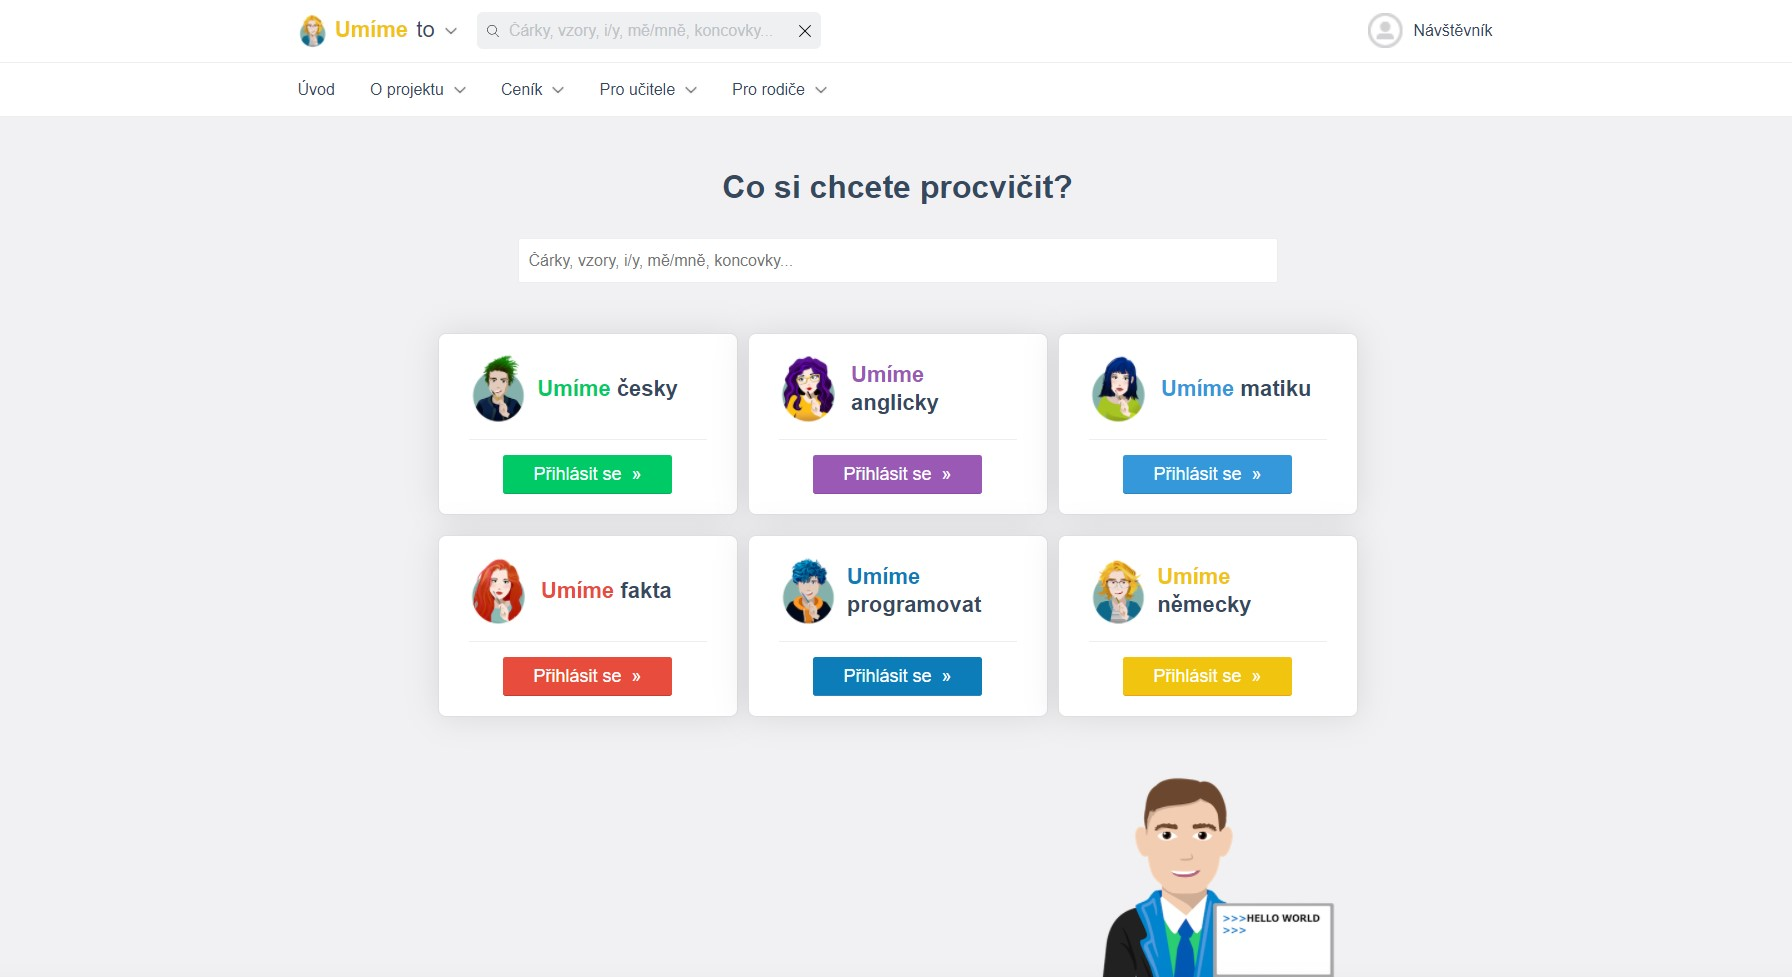
\includegraphics[width=\textwidth]{images/umimeto}
    \label{img:umimeto}
\end{figure}

Výhody:
\begin{itemize}
  \item Hezké a čisté uživatelské rozhraní.
  \item Velká spousta předpřipravených úkolů různých typů
\end{itemize}

Nedostatky:
\begin{itemize}
  \item Omezení jen na předpřipravené úlohy
  \item Málo statistik
  \item Registraci a připojení ke třídě si musí řešit žáci sami
  \item Chybějící chat
\end{itemize}


%\subsection{Classkick - TODO}

\section{Shrnutí}

Z předchozích implementací vychází několik poznatků, které bych zde rád shrnul.

V první řadě většina z nich je příliš složitá pro žáky prvního stupně. Svou implementaci bych tedy měl směřovat hlavně k tomu, aby byla jednoduchá, intuitivní a přehledná.

S tím souvisí další častý problém s registracemi. Bude mnohem jednodušší, když si žáky přidá do třídy rovnou učitel a žáci se pak jen přihlásí uživatelským jménem, které jim je sděleno a zvolí si pouze své heslo.

To samé by mohlo platit i pro samotné učitele a třídy. Ty bude registrovat a vytvářet administrátor a rovnou je k sobě přiřadí. Učitel se tedy jen přihlásí a zvolí si pouze své heslo stejně jako žák. Tím nemusí nic dalšího řešit a může jít rovnou vytvořit účty žákům.

Dále bude potřeba propracovat zadávání a odevzdávání úkolů. Mělo by platit, že zadání může měnit pouze učitel a žák k němu posílá pouze své řešení. To může následně učitel vrátit k přepracování s komentářem, ovšem nesmí upravovat žákovo řešení, aby ho například omylem nesmazal.

Všichni uživatelé musí jasně vidět přehled toho, co musí ještě udělat. Pokud tedy například žák odešle řešení úkolu, tak by se měl tento úkol rovnou přesunout do méně důležité sekce, aby se nepletl s aktuálními povinnostmi.

Snadné by také mělo být přepínání mezi předměty (v případě učitele i mezi třídami).

Vhodnou funkcí je i třídní chat. Ideálně pro každý předmět zvlášť.